\documentclass[]{beamer}
\mode<presentation>
{
  \usetheme{Warsaw}
  \definecolor{mcgarnet}{rgb}{0.38, 0, 0.08}
  \definecolor{mcgray}{rgb}{0.6, 0.6, 0.6}
  \setbeamercolor{structure}{fg=mcgarnet,bg=mcgray}
  %\setbeamercovered{transparent}
}


\usepackage[english]{babel}
\usepackage[latin1]{inputenc}
\usepackage{times}
\usepackage[T1]{fontenc}
\usepackage{tikz}
\usepackage{graphicx}
\usepackage{adjustbox}
\usepackage{fancyvrb}

\newcommand{\imagesource}[1]{{\centering\hfill\break\hbox{\scriptsize Image Source:\thinspace{\small\itshape #1}}\par}}

\title{05 - Making Decisions - Part 1}


\author{Dr. Robert Lowe\\}

\institute[Maryville College] % (optional, but mostly needed)
{
  Division of Mathematics and Computer Science\\
  Maryville College
}

\date[]{}
\subject{}

\pgfdeclareimage[height=0.5cm]{university-logo}{images/Maryville-College}
\logo{\pgfuseimage{university-logo}}



\AtBeginSection[]
{
  \begin{frame}<beamer>{Outline}
    \tableofcontents[currentsection]
  \end{frame}
}


\begin{document}

\begin{frame}
  \titlepage
\end{frame}

\begin{frame}{Outline}
  \tableofcontents
\end{frame}


% Structuring a talk is a difficult task and the following structure
% may not be suitable. Here are some rules that apply for this
% solution: 

% - Exactly two or three sections (other than the summary).
% - At *most* three subsections per section.
% - Talk about 30s to 2min per frame. So there should be between about
%   15 and 30 frames, all told.

% - A conference audience is likely to know very little of what you
%   are going to talk about. So *simplify*!
% - In a 20min talk, getting the main ideas across is hard
%   enough. Leave out details, even if it means being less precise than
%   you think necessary.
% - If you omit details that are vital to the proof/implementation,
%   just say so once. Everybody will be happy with that.

\section{Branching}

\begin{frame}{Introduction to Branching}
    \begin{itemize}[<+(1)->]
        \item Branching is when a program selects between multiple
            paths of execution.
        \item Programs make choices according to statements which are
            either true or false.
    \end{itemize}

    \begin{block}{What is Truth?}<+(1)->
        \uncover<+(1)->{In C++, 0 is false.  All other values are true.}
        \newline\uncover<+(1)->{We usually use expressions which
            logically evaluate to true or false as conditions}
    \end{block}
\end{frame}

\begin{frame}{Comparison Operations}
    \uncover<+->{\textbf{Relational Operators}}
    \begin{description}[<+->]
        \item[\texttt{<}] Less Than
        \item[\texttt{>}] Greater Than
        \item[\texttt{<=}] Less Than or Equal To
        \item[\texttt{>=}] Greater Than or Equal To
    \end{description}

    \uncover<+->{\textbf{Equality Operators}}
    \begin{description}[<+->]
        \item[\texttt{==}] Equal
        \item[\texttt{!=}] Not Equal
    \end{description}
\end{frame}

\begin{frame}{Operator Precedence (Thus Far)}
    \begin{tabular}{|l|l|l|}
        \hline
        \textbf{Operator} & \textbf{Description} & \textbf{Associativity} \\
        \hline
        \texttt{a*b}, \texttt{a/b}, \texttt{a\%b} & Multiply, Divide, Modulus & Left-to-Right\\
        \hline
        \texttt{a+b}, \texttt{a-b} & Addition and Subtraction & Left-to-Right\\
        \hline
        \texttt{<<} , \texttt{>>} & Insertion and Extraction & Left-to-Right \\
        \hline
        \texttt{<}, \texttt{<=} & Relational Operators & Left-to-Right\\
        \texttt{>}, \texttt{>=} & & \\
        \hline
        \texttt{==}, \texttt{!=} & Equality Operators & Left-to-Right\\
        \hline
        \texttt{=},  & Assignment and Assignment & Right-to-Left \\
        \texttt{+=}, \texttt{-=} & & \\
        \texttt{*=}, \texttt{/=} & & \\
        \texttt{\%=} & & \\
        \hline
    \end{tabular}
\end{frame}

\begin{frame}[fragile]{If Statement}
\begin{columns}
    \column{0.5\textwidth}
    \verb!if(! \textit{condition} \verb!)! 
    \verb!    ! \textit{statement/block}

    \vspace{2cm}

    \begin{itemize}[<+(1)->]
        \item If the \textit{condition} is true, the
            \textit{statement/block} will be executed.
        \item If the \textit{condition} is false, the 
            \textit{statement/block} will be skipped.
    \end{itemize}

    \column{0.5\textwidth}
    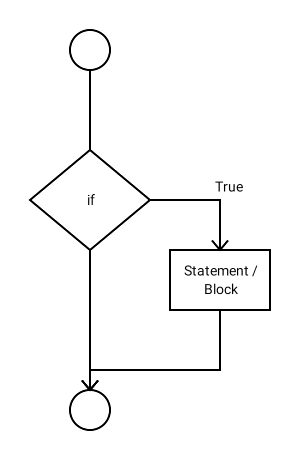
\includegraphics[width=0.9\textwidth]{images/if}
\end{columns}
\end{frame}

\begin{frame}[fragile]{Example: \texttt{even.cpp}}
\begin{adjustbox}{max height=0.9\textheight, max width=0.95\textwidth}
\begin{BVerbatim}
int main()
{
    int num;  //the number to test

    //get the number
    cout << "Enter a number: ";
    cin >> num;

    //inform the user if it is even
    if( num % 2 == 0 ) {
        cout << "The number " << num << " is even" << endl;
    }
}
\end{BVerbatim}
\end{adjustbox}
\end{frame}

\begin{frame}[fragile]{If Else Statement}
\begin{columns}
    \column{0.5\textwidth}
    \verb!if(! \textit{condition} \verb!)! 
    \newline\verb!    ! \textit{then statement/block}
    \newline\verb!else!
    \newline\verb!    ! \textit{else statement/block}

    \vspace{1cm}

    \begin{itemize}[<+(1)->]
        \item If the \textit{condition} is true, the
            \textit{then statement/block} will be executed.
        \item If the \textit{condition} is false, the 
            \textit{else statement/block} will be executed.
    \end{itemize}

    \column{0.5\textwidth}
    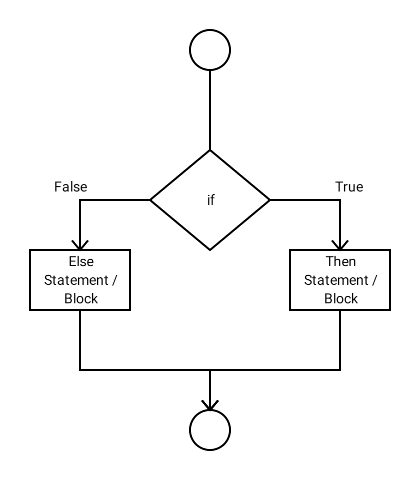
\includegraphics[width=0.9\textwidth]{images/if-else}
\end{columns}
\end{frame}

\begin{frame}[fragile]{Example: \texttt{even-odd.cpp}}
\begin{adjustbox}{max height=0.9\textheight, max width=0.95\textwidth}
\begin{BVerbatim}
int main()
{
    int num;  //the number to test

    //get the number
    cout << "Enter a number: ";
    cin >> num;

    //inform the user if it is even or odd 
    if( num % 2 == 0 ) {
        cout << "The number " << num << " is even" << endl;
    } else {
        cout << "The number " << num << " is odd" << endl;
    }
}
\end{BVerbatim}
\end{adjustbox}
\end{frame}

\begin{frame}[fragile]{Best Practices}
    \begin{itemize}[<+->]
        \item Curly braces are optional, but always use them.

        \item Do this:
        \newline\begin{BVerbatim}
if( x == 1 ) {
    cout << "Yes, x is 1" << endl;
}
        \end{BVerbatim}

        \item Not this:
        \newline\begin{BVerbatim}
if( x == 1 ) 
    cout << "Yes, x is 1" << endl;
        \end{BVerbatim}

        \item Be consistent about brace styles!

        \item Always indent the contents of the if's block.
    \end{itemize}
\end{frame}


\section{Thinking With Branches}
\begin{frame}{Pythagoras}
\begin{columns}
    \column{0.6\textwidth}
    \begin{itemize}[<+->]
        \item Pythagoras lived in Croton around 500 BC.
        \item Taught that everything could be quantified by whole
            units (integers).
        \item Founded a mystery cult, called the Pythagoreans.
        \item The Pythagoreans kept all their math secret.
        \item The Pythagoreans died under siege by burning themselves
            to death on a funeral pyre made of their mathematical works.
    \end{itemize}

    \column{0.4\textwidth}
    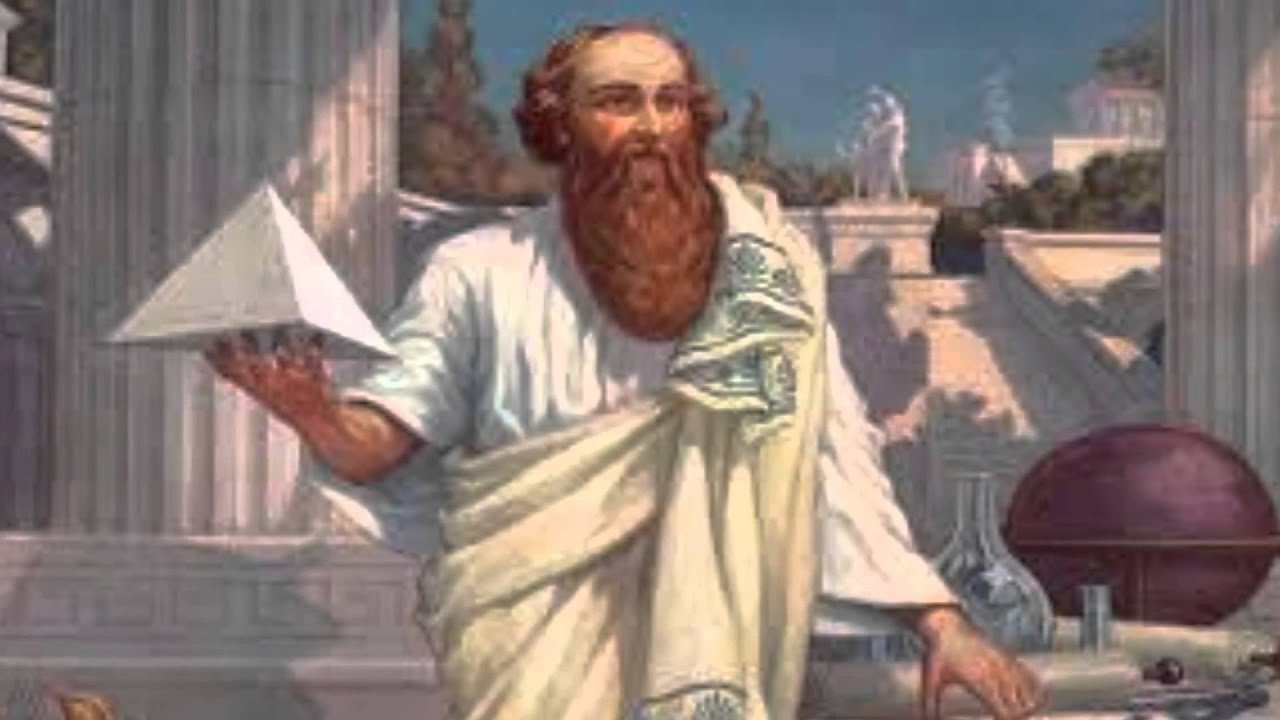
\includegraphics[width=0.95\textwidth]{images/pythagoras}
    \newline{\tiny URL: \url{https://www.youtube.com/watch?v=Vn4rwks1eMk}}
\end{columns}
\end{frame}

\begin{frame}{The Problem}
    One day, a student discovered that irrational numbers necessarily
    exist, even in simple observable shapes!
    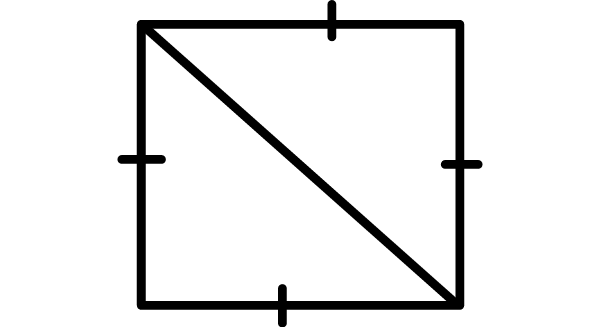
\includegraphics[width=0.9\textwidth]{images/Irrational}
\end{frame}

\begin{frame}{The Solution}
    This caused Pythagoras a lot of distress.
    \newline\uncover<2->{Luckily, his students found a solution!}

    \uncover<3->{
        \begin{center}
        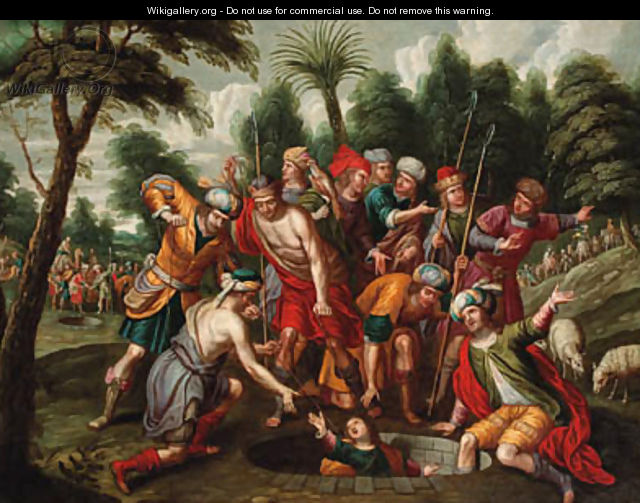
\includegraphics[height=0.65\textheight]{images/well}
        \newline{\tiny Image Source:
        \url{http://www.wikigallery.org/wiki/painting_285033/Peeter-Sion/Joseph-lowered-into-the-well-by-his-brothers}}
        \end{center}
    }
\end{frame}

\begin{frame}{The Real Solution}
    \begin{center}
        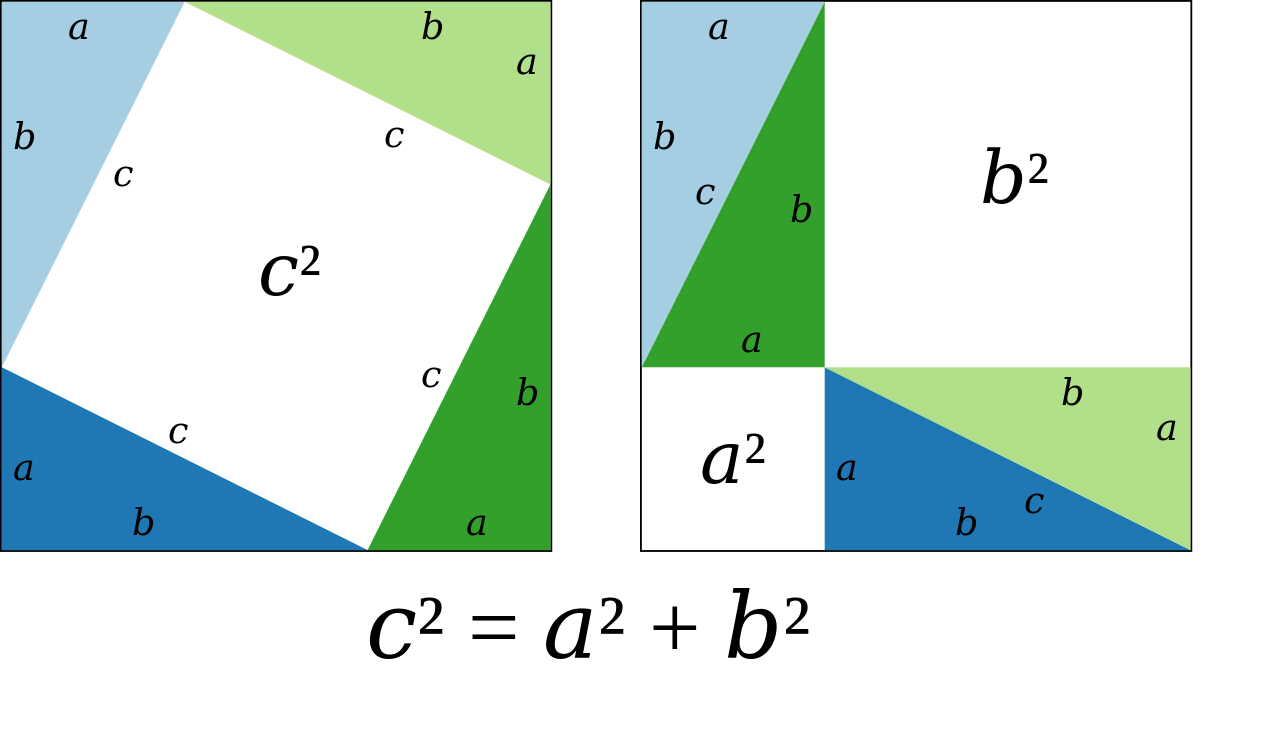
\includegraphics[width=0.95\textwidth]{images/pythagoras-proof}
        \newline{\tiny Image Source: \url{https://commons.wikimedia.org/wiki/File:Pythagoras-proof-anim.svg}}
    \end{center}
\end{frame}

\begin{frame}[fragile]{Pythagoras Design}

    Let's design a program that can compute any side of a right
    triangle! 

        It can find a leg:
\begin{verbatim}
I know how to find: 
  1.) A Leg
  2.) A Hypotenuse
Which do you want? 2
A=3
C=5
A=3
B=4
C=5
\end{verbatim}
\end{frame}

\begin{frame}[fragile]{Pythagoras Design}
        It can find the hypotenuse:
\begin{verbatim}
I know how to find: 
  1.) A Leg
  2.) A Hypotenuse
Which do you want? 2
A=3
B=4
A=3
B=4
C=5
\end{verbatim}
\end{frame}

\begin{frame}[fragile]{\texttt{pythagoras.cpp}: Variables}
\begin{verbatim}
    double a, b, c;  //triangle sides
    int choice;      //the user's choice
\end{verbatim}
\end{frame}

\begin{frame}[fragile]{\texttt{pythagoras.cpp}: Getting the Choice}
\begin{verbatim}
    //get the user's choice
    cout << "I know how to find: " << endl
         << "  1.) A Leg" << endl
         << "  2.) A Hypotenuse" << endl
         << "Which do you want? ";
    cin >> choice;
\end{verbatim}
\end{frame}

\begin{frame}[fragile]{\texttt{pythagoras.cpp}: Making the Decision}
\begin{verbatim}
    //perform the user's choice
    if(choice == 1) {
        //find a leg
    } else {
        //find the hypotenuse
    }
\end{verbatim}
\end{frame}

\begin{frame}[fragile]{\texttt{pythagoras.cpp}: Find a Leg}
\begin{verbatim}
        //get A and C
        cout<< "A=";
        cin >> a;
        cout << "C=";
        cin >> c;

        //solve for b
        b = sqrt(c*c - a*a);
\end{verbatim}
\end{frame}

\begin{frame}[fragile]{\texttt{pythagoras.cpp}: Find the Hypotenuse}
\begin{verbatim}
        //get A and B
        cout << "A=";
        cin >>  a;
        cout << "B=";
        cin >> b;

        //solve for c
        c = sqrt(a*a + b*b);
\end{verbatim}
\end{frame}


\begin{frame}[fragile]{\texttt{pythagoras.cpp}: Display the Results}
\begin{verbatim}
    //print the results
    cout << "A=" << a << endl
         << "B=" << b << endl
         << "C=" << c << endl;
\end{verbatim}
\end{frame}


\begin{frame}{Challenge: Modify \texttt{quadratic.cpp}}
    Make the following changes to the behavior of the quadratic
    program we wrote last time.
    \begin{enumerate}
        \item Only display the roots if the equation has real roots.
        \item If there are no real roots of the equation, display the
            message "No real roots."
        \item If both roots are the same, only display one root. (Do
            not repeat roots.)
    \end{enumerate}
\end{frame}

\begin{frame}{Week 3 Lab Requirements}

    For full credit you must have:
    \begin{enumerate}
        \item \texttt{circle.cpp}
        \item \texttt{pythagoras.cpp}
        \item \texttt{quadratic.cpp} (as modified on the previous
        slide).
    \end{enumerate}

    Be sure to add, commit, and push!
\end{frame}


\end{document}


